The main result of this paper is that we can approximately compute $\bn_{MAP}$ in \emph{linear} time, whereas an exact solution would require exponential time. Fig. \ref{fig:schem} shows an example of running the FANSI filter on simulated data.  The top three panels show $bF$, $\bC$, and $\bn$, simulated according to our model, Eqs. \eqref{eq:F} and \eqref{eq:C}.  The bottom panel shows the output of our FANSI filter.  Note that the FANSI filter does not provide the most likely spike train, $\bn_{MAP}$, but rather an approximation to it, $\tbn$ (see Eq. \eqref{eq:obj2} for definition), that is computable exactly in \emph{linear} time.  



%\begin{figure}[H]
%\centering 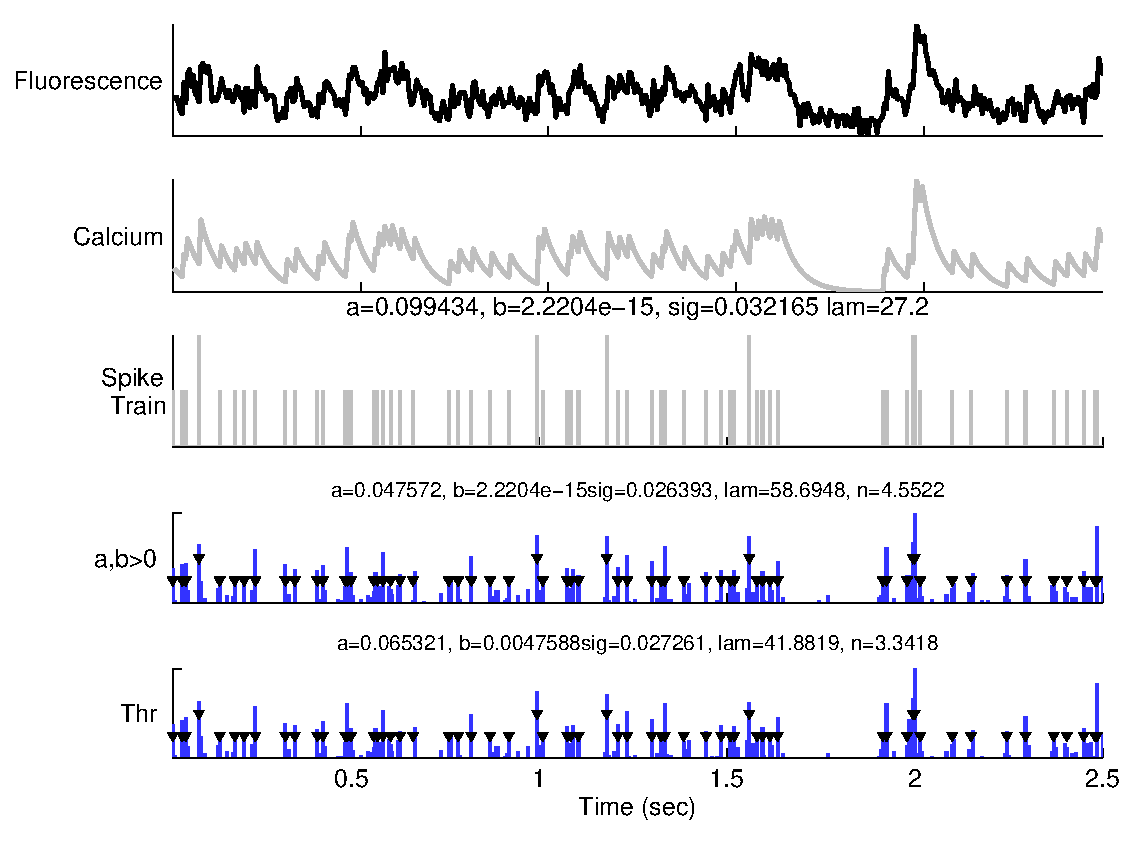
\includegraphics[width=.9\linewidth]{schem}
%\caption{Simulation demonstrating our neuron model and inference. Note that the effective signal-to-noise ratio (SNR) of our FANSI filter improves on the Wiener filter, largely by eliminating the ringing effect present in the Wiener filter output.  For both filters, only the fluorescence was provided to the algorithm, so both the parameters and the inference were performed using this minimal amount of data.  Top panel: Simulated fluorescence. Second panel: Simulated intracellular calcium concentration. Third panel: Simulated spike train.  Fourth panel: Wiener filter (blue for positive inference, red for negative), superimposed on simulated spike train (black triangles).  Bottom panel: Fast filter (same conventions as fourth panel). Parameters:  $\gamma=0.94$, $\nu=0$, $\rho=1$, $\sig=0.3$, $\lam=8$, $\Del=0.005$ msec.} \label{fig:schem2}
%\end{figure}

According to the above model (Eq. \eqref{eq:C}), the neuron spikes according to a Poisson distribution, which is well approximated by an exponential distribution, when the rate is low.  However, when the rate is high, e.g., several spikes per time bin, the distribution of spikes would be better approximated by a Gaussian distribution.  The optimal linear filter, upon making this assumption, is typically called a Wiener filter \cite{Wiener49}.\footnote{See Appexdix \ref{sec:wiener} for a derivation of the Wiener filter for this model.}  Importantly, the Wiener admits negative spikes as viable solutions, as a Gaussian distribution has support on the entire real number line (our FANSI filter, however, imposes a non-negative constraint).  Thus, a natural question to ask is how our FANSI filter compares with the Wiener filter on both slow and fast spike trains.  Figure \ref{fig:wiener} depicts the performance of both the FANSI filter and Wiener filter for these two scenarios: the top panels show the fluorescence traces provided to the two filters, the middle panel shows the outputs of the FANSI filter, and the bottom panel shows the outputs of the Wiener filter.

On the left, it is clear that the FANSI filter significantly outperforms the Wiener filter, in terms of signal-to-noise ratio (SNR).  Specifically, the Wiener filter infers \emph{negative} spikes throughout the time course, resulting in the so-called ``ringing'' effect.  Intuitively, the ringing results from the most likely explanation of a strong downward shift in fluorescence is a corresponding downward shift in spiking.  The FANSI filter prohibits downward spiking events (with the non-negative constraint), and therefore, does not suffer from ringing.  

On the right, both filters seem to perform very well, suggesting that even when the true spike distribution is better approximated by a Gaussian distribution, the exponential distribution is sufficient.  Because the Wiener filter \nai vely requires $O(T \log T)$, whereas the FANSI filter requires only $O(T)$, this suggests that the FANSI filter performs both (i) at least as well, and (ii) faster than the Wiener filter.  

%$, and a na\"{i}ve approximate solution would require polynomial time.
%
%When the observed neuron is spiking quickly, the Poisson distribution may be well approximated by a Gaussian distribution, suggesting that the Wiener filter may be optimal in this regime.  But the exponential approximation of a Poisson is also very accurate in the fast spiking regime.  To compare these two strategies, we simulated a fast spiking neuron, where the expected number of spikes per bin exceeds 10 (Fig. \ref{fig:FastSpiking}). In this scenario, both the Wiener filter and our FANSI filter perform approximately equally well.  Both filters infer peaks in the firing rate that are obscured by the low-pass filter properties of the calcium dynamics. Thus, it seems from this analysis that regardless of the firing rate of the observable neuron, (1) filtering the signal may provide valuable information, and (2) our FANSI filter performs at least as well as the Wiener filter, without requiring more computational time.
%
%To evaluate the efficacy of our FANSI filter, we compare it with the optimal linear (i.e., Wiener) filter \cite{Wiener49}. The top three panels of Fig. \ref{fig:schem} depict a typical dataset simulated according to our model, Eqs. \eqref{eq:obs} and \eqref{eq:trans}. Beneath the simulation, we show both the Wiener filter output (fourth panel) and our FANSI filter output (bottom panel).  For both filters, we provided only the fluorescence observations depicted in the top panel, and $\ve{\eta}$.  From this data, we estimate the remaining parameters, and infer the hidden spike train. Several differences between these two approaches should be apparent.  First, the effective signal-to-noise ratio (SNR) of our FANSI filter improves upon the optimal linear filter.  Second, while the Wiener filter induces a ``ringing'' effect (where the inferred signal oscillates above and below zero), our FANSI filter completely eliminates this effect.  These two improvements are common observations upon imposing a non-negative constraint when appropriate \cite{ShumwayStoffer06}.  Importantly, both our implementation of the Wiener filter and our FANSI filter require only $O(T)$ time, whereas the na\"{i}ve implementation of the Wiener filter requires $O(T \log(T))$, and the na\"{i}ve implementation of a non-negative filter requires $O(T^3)$.  Thus, when our approximation in Eq \eqref{eq:obj2} is good, our filter outperforms the Wiener filter, and imposes approximately the same computational burden.

\begin{figure}[H]
\centering 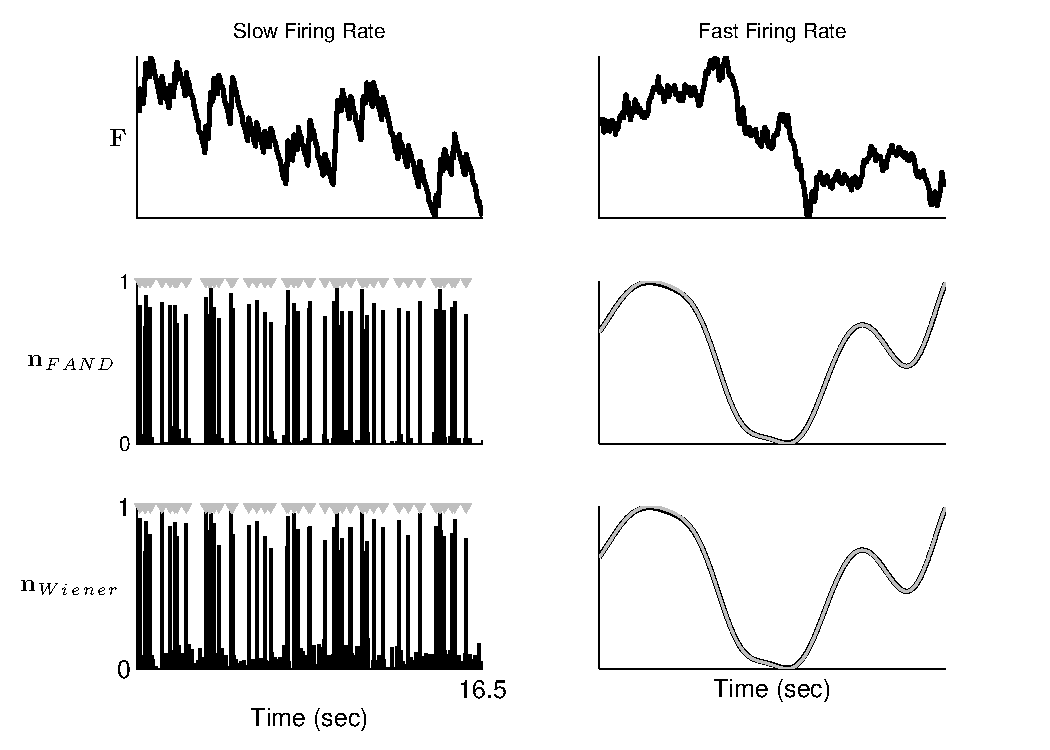
\includegraphics[width=.9\linewidth]{../figs/wiener}
\caption{A simulation demonstrating that the FANSI filter performs at least as well as the optimal linear (i.e., Wiener) filter. The left panels show that in the slow firing regime, the FANSI filter outperforms the Wiener filter in terms of SNR.  This ``makes sense'', given that if a neuron is spiking according to a Poisson distribution with a slow rate, an exponential distribution is a better approximation than a Gaussian distribution, and the FANSI filter approximates the spike train distribution with an exponential, versus the Wiener filter's Gaussian. The right panels show that both approximations are sufficient in the fast firing regime. Top left panel: fluorescence time series for a neuron with a slow firing rate.  Middle left panel: the FANSI filter's inferred spike train.  Bottom left panel: Wiener filter's inferred spike train.  Note that (i) the Wiener filter does not impose a non-negativity constraint, and (ii) the effective SNR of the Wiener filter in this example is worse than the FANSI filter's.  Top right panel: same as top left panel, for a neuron with a high firing rate.  Middle right panel: the FANSI filter's inferred spike train smoothed with a Gaussian kernel for visualization purposes (black line), and the true spike train smoothed with the same Gaussian kernel (gray line).  Bottom right panel: same as middle right panel, but with the Wiener filter. Parameters for left panels: same as above.  Parameters for right panels: same as above, except: $\sig=8$ photons, $\lam=500$ Hz.} \label{fig:wiener}
\end{figure}

%\newpage \begin{figure}[H]
%\centering 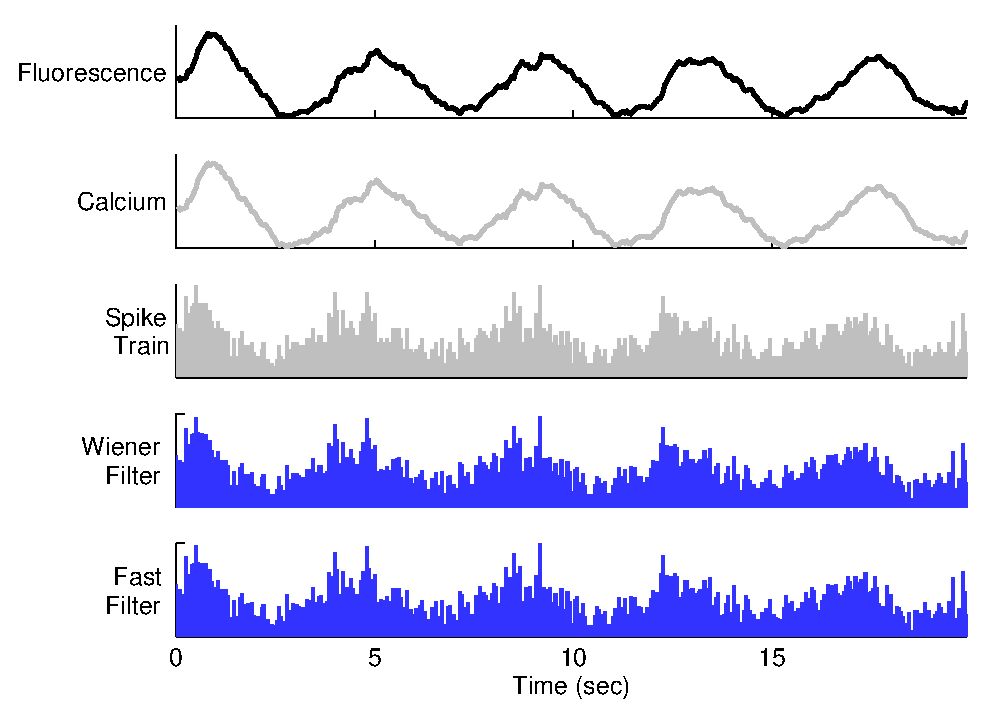
\includegraphics[width=.9\linewidth]{FastSpiking}
%\caption{Comparing the Wiener filter and our FANSI filter for a fast spiking neuron.  In this scenario, the two filters perform approximately equally well. Note that both recover fast fluctuations in the firing rate that are smoothed out by the calcium dynamics. Conventions as in Fig. \ref{fig:schem}.  Actual and inferred spike trains were normalized similarly, to ease comparisons. Parameters: $\gamma=0.94$, $\nu=0$, $\rho=1$, $\sig=0.3$, $\lam=100$ (modulated by a sinusoid), $\Del=0.05$ msec.} \label{fig:FastSpiking}
%\end{figure}


